\documentclass[useAMS,natbib]{mn2e}
\usepackage{epsfig}
\usepackage{amssymb}
\usepackage{amsmath}
\usepackage{graphicx, import}
\graphicspath{ {Images/} }
\bibliographystyle{apalike2}

%=\usepackage[square,sort,comma,numbers]{natbib}
\usepackage{hyperref}
\newcommand\ion[2]{#1\,{\scshape{#2}}}%                       % ion, i.e., CII = \ion{C}{ii}

% If your system does not have the AMS fonts version 2.0 installed, then
% remove the useAMS option.
%
% useAMS allows you to obtain upright Greek characters.
% e.g. \umu, \upi etc.  See the section on "Upright Greek characters" in
% this guide for further information.
%
% If you are using AMS 2.0 fonts, bold math letters/symbols are available
% at a larger range of sizes for NFSS release 1 and 2 (using \boldmath or
% preferably \bmath).
%
% The usenatbib command allows the use of Patrick Daly's natbib.sty for
% cross-referencing.
%
% If you wish to typeset the paper in Times font (if you do not have the
% PostScript Type 1 Computer Modern fonts you will need to do this to get
% smoother fonts in a PDF file) then uncomment the next line
% \usepackage{Times}

%%%%% AUTHORS - PLACE YOUR OWN MACROS HERE %%%%%


%%%%%%%%%%%%%%%%%%%%%%%%%%%%%%%%%%%%%%%%%%%%%%%%

\title[Measuring Column Density of Neutral Hydrogen near the Galactic Center of the Milky Way] {Simulating the atmospheres of Titan and Pluto using Microphysics}
\author[Jesus Javier Serrano]{Jesus Javier Serrano\thanks{E-mail:
jjserran@ucsc.edu}\\
\\Department of Astronomy and Astrophysics, University of California, Santa Cruz, CA 95064
}

\begin{document}

\date{3/18/19}

\pagerange{\pageref{firstpage}--\pageref{lastpage}} \pubyear{2019}

\maketitle

\label{firstpage}

\begin{abstract} % Was 201 words
Within the past century, direct observations of Titan's and Pluto's atmosphere have proven their composition to be alike. Ever since then several physical models have been tested on Earth in order to simulate the interactions between organic molecules present within these planets' atmospheres. This investigation two separate mathematical models were analyzed with the purpose of understanding the statistical dynamics occuring within these atmospheres. Both models have proven inaccurate with current observations but show a good boundary towards expected values of physical parameters for lower atmosphere regimes.
\end{abstract}


\section{Introduction} % Section 1
\indent~~In 2017, the Cassini mission came to an end after providing sufficient amount of data regarding Titan's atmosphere. Cassini was able to observe the brightness profile of the atmosphere within the Infrared range which provided a precise measurement of the organic composition within the atmosphere. Along with Cassini's observations, Voyager 1 and 2 both offered measurements of organic compositions within Titan's atmosphere which helped classified Titan as a model for pre-biotic Earth.\cite{TitanVerticalAerosol}\\
\indent~~Titan's atmosphere provided insight as to how gaseous organic atmospheres affect the temperature of the planet. With a significant amount of observations and physical models made in order to understand Titan's atmosphere, Titan was soon used as a comparison model for any planet containing organic atmospheres. This provided an insight into the composition of Pluto's atmosphere. On June 9th, 1988, NASA's Kuiper Airborne Observatory (KAO) captured the stellar occultation made by Pluto which showed an extinction layer present along more than half of Pluto's circumference. It was known that Pluto contained organic ice and Nitrogen ice with a similar relative abundance to that of Titan's atmosphere, and Pluto's surface temperature which ranges from $35-40 K$ is enough to sublimate the ice. Thus, the occultation provided possible evidence for a thin atmosphere with a composition that was similar to that of Titan.\\
\begin{figure}
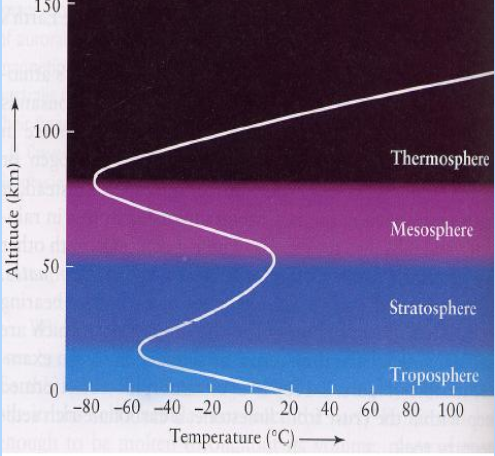
\includegraphics[scale = 0.6]{earth_temp}
\includegraphics[scale = 0.45]{Titan_temp}
\caption{Earth's temperature profile (top) and Titan's temperature profile (bottom) both show similar trends as seen within the troposphere and Mesosphere in each of these planet's regimes. Notice the concavity trends on both temperature profiles are alike with a small increase in temperature within the mesosphere for Titan compared to Earth.}
\label{temp}
\end{figure}
\indent~~In 2015 New Horizons provided a direct observation of the optically thin Haze layers present within the first few $km$ above the surface of Pluto. These organic haze layers along with Titan's abundance of Methane, although being directly observed to a significant degree, are improbable results if the only assumptions applied are ideal gases with an upwards Jean's flux being present from the photo-dissociation of organic molecules. Thus, a consistent model for these atmospheres must include a different system of dynamical constraints aside from chemical interactions and radiative process which dominate the upper and lower layers of the atmosphere. In order to account for the dynamics present within the haze layers of Pluto and organic layers of Titan, microphysics must be applied which is defined as a mixture of statistical mechanics and fractal dynamics. Two models were proposed and fitted to the observations of both Titan and Pluto in order to account for the micro-physics present in these systems. Panayotis Lavvas applied a constraint model of coagulation onto Titan's atmosphere in order to mimic the temperature profile observed. Peter Gao applied a similar model to Lavvas but applied weights to characterize the coagulation present in the thin haze of Pluto. These two models were alike due to the fact that Titan and Pluto have similar atmospheric composition and thus the assumption that both systems must have similar constraints was applied.\\
\section{Statistical Modeling with Coagulation}
\subsection{Titan's Model}
\begin{figure}
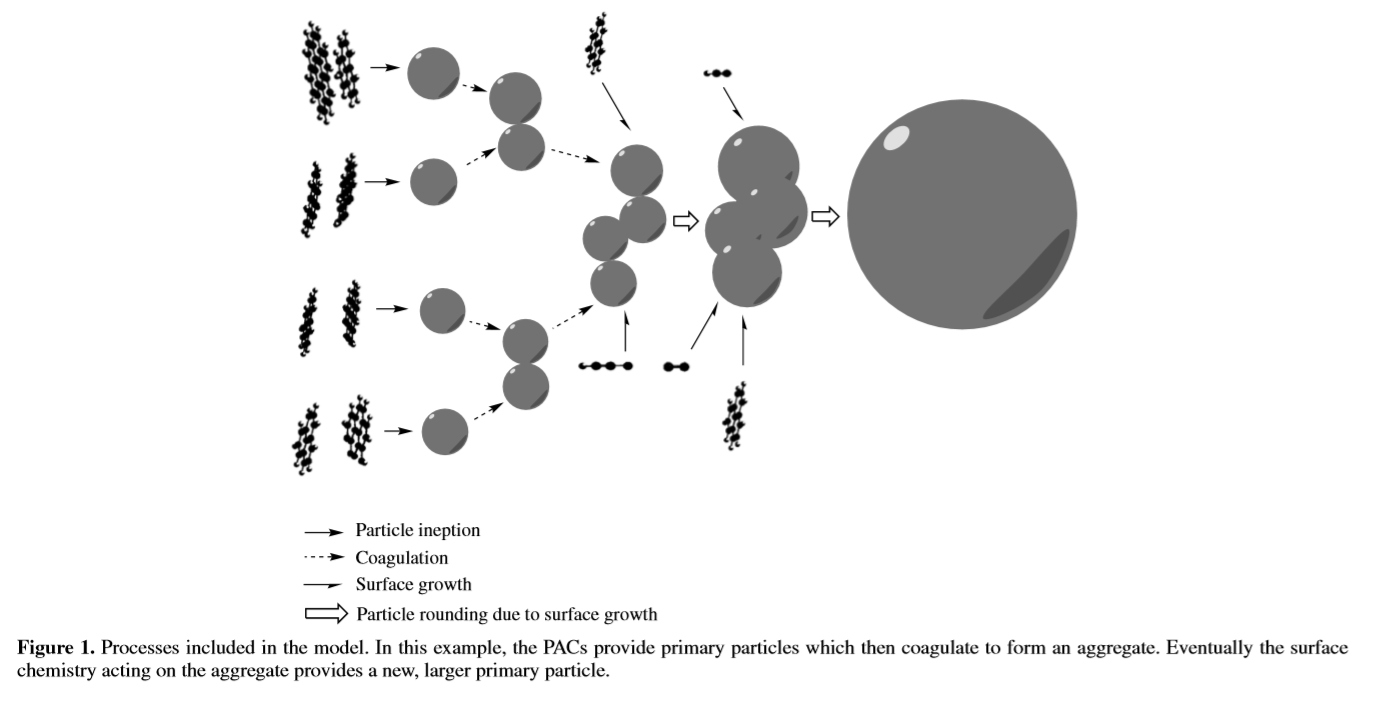
\includegraphics[scale = 0.3]{coagulation}
\caption{Model of Coagulation showing how small cyclic compounds inelastically combine to form large PAC structures}
\label{coag}
\end{figure}
\indent~~Lavvas approach was to append a continuity equation onto the flux movement of the coagulated particles in the atmosphere. Titan's model was built upon the movement of polycyclic aromatic compounds (PAC) within the atmosphere which grow when attached to other compounds into larger bodies. The coagulation process starts with a cyclic organic compound which chemically reacts with radicals abundant in the atmosphere. These radicals create fractal-like structures with the cyclic ring and thus inelastic collisions are more probable to happen. The radically modified cyclic ring then binds with other organic structures in the atmosphere an grow in both mass and size. This creates a hierarchy of polycyclic compounds with different mass regimes $m_i$ and volumetric radii $r_i$ This entire process of binding radically modified cyclic rings is defined as coagulation and it dependent upon surface growth and sedimentation. A mathematical model of the movement of coagulates between different mass regimes is characterized by the aerosol continuity equation which is defined on \textbf{Equation} \ref{cont}.
\begin{figure}
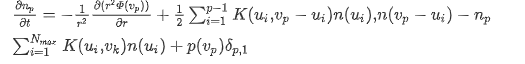
\includegraphics[scale = 0.6]{aerosel_cont}
\caption{The aerosol equation is defined as the change in time $t$ of the number density $n_p$ within a certain mass regime $m_i$ is equal to the difference between the incoming flux of coagulates from the smaller regimes and a photochemical production quantity $p(v_p)$ minus the outgoing flux of the coagulates within $m_i$ that grow into larger mass regimes and the radial divergence of the coagulate flux $\Phi(v_p)$ with volume $v_p$. Note that $\Phi(v_p)$ is dependent upon sedimentation and eddy mixing.}
\label{cont}
\end{figure}
The $K$ components present in the aerosol continuity equations are defined as coagulation kernel and are matrix components which define the rate of coagulation within a certain transition between two volume regimes $u_i$ and $v_p - u_i$. These kernels are modeled using Brownian motion and can be approximated using both low and high pressure limit boundaries for these kernels. From the aerosol equation a model was built by applying a limited set of radicals used to build the PAC mass regimes. These radicals were determined both experimentally and theoretically using photochemical models, which is shown on \textbf{Figure} \ref{rad}.\\
\begin{figure}
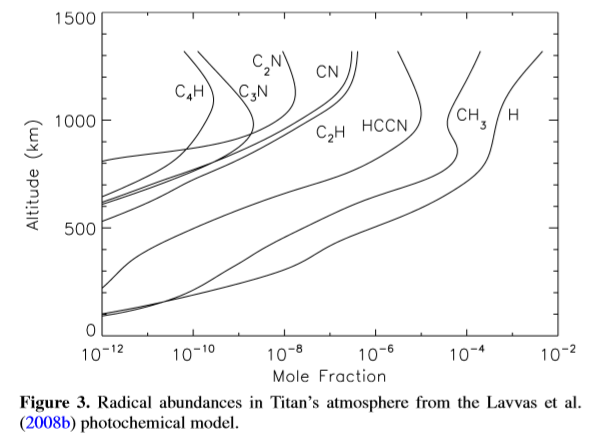
\includegraphics[scale = 0.6]{rad_abund}
\caption{Abundance of radicals present in Titan's atmosphere using a photochemical model simulation built by Lavvas}
\label{rad}
\end{figure}
\indent~~From the model flux of coagulates defined in the continuity equation, a set of physical parameters known about Titan's atmosphere was applied into a Runga-Kuta 4 Monte Carlo simulation in order to calculate the particle column density and physical parameters of the PAC's as a function of height.
\subsection{Pluto's Model}
Peter Gao provided a similar model to Pluto in which the aerosol continuity equation was used to to approximate movement of coagulated monomers due entirely to sedimentation. Thus defining the flux of coagulates within a certain mass regime as being dependent upon purely on eddy diffusion. Also, since Gao is using monomers instead of cyclic organic compounds then the fractal geometry and therefore dynamics of the model differs due to the difference in mass and volume definition for each coagulate. A weighted model was applied to the flux so as to approximate the fractal geometry of monomers as porous spheres. Gaos also accounted for the physical drag caused by charge and viscosity and related the eddy diffusion to these parameters. The resulting model compared purely spherical coagulates to aggregated coagulates in order to define the boundaries of expected observation data in terms of particle density as a function of altitude.
\begin{figure}
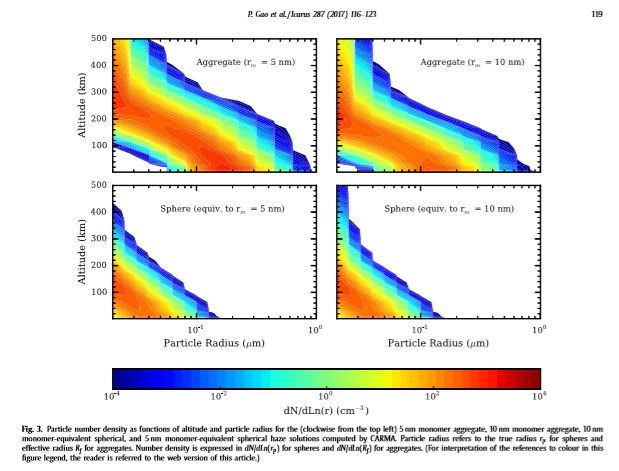
\includegraphics[scale = 0.5]{particle_density_shape}
\caption{Peter Gaos model representing the particle density as a function of shape and altitude.}
\label{part_shape}
\end{figure}
\section{Agreement with Observations}
\indent~~Lavvas applied the coagulation model of PAC's onto Titan observations and found that the model resulted in a relatively small aerosol mass flux which is one order of magnitude lower than observation. Peter Gao also found difficulty in fitting the model to observations made on Pluto's atmosphere. The extinction coefficient approximated on Pluto by Gao was approximate and was able to apply a boundary to observations within the spherical and aggregate model regime. Gao's model is shown on \textbf{Figure} \ref{ext_pluto}. Further investigation is needed upon the coupling of several dynamical influencing the coagulation process and the particle flux in the atmosphere. \\
\begin{figure}\centering
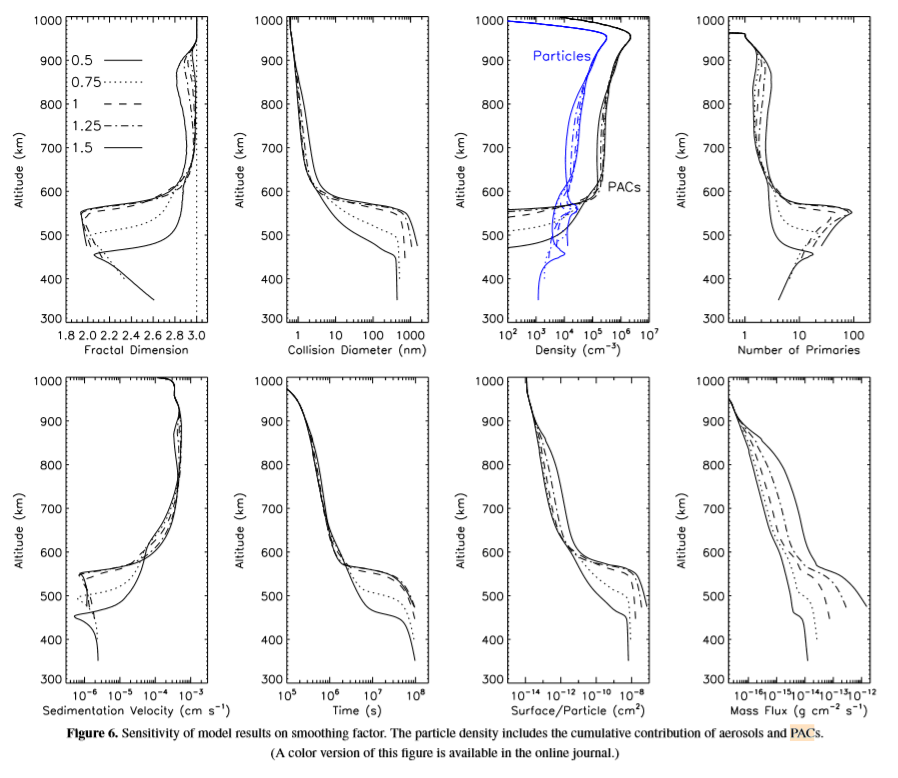
\includegraphics[scale = 0.4]{titan_model}
\caption{Note that the individual particle model results in a smaller magnitude of number density when compared to the PAC model of coagulates.}
\label{tit_model}
\end{figure}
\begin{figure}\centering
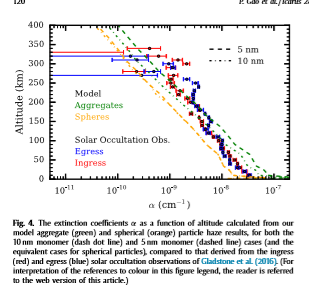
\includegraphics[scale = 0.6]{extinction_pluto}
\caption{The spherical and aggregate particles create a strong boundary for the observations made by New Horizons. Note that the aggregate model agrees with observation on the top half of the atmosphere and the spherical model agrees with the lower half.}
\label{ext_pluto}
\end{figure}
\section{Conclusion}
Lavvas proposed that even though the model was not able to fit to direct observvations of Titan's atmosphere at high altitudes, it is possible that model can be best fitted to lower atmosphere observations. Thus the pure coagulation process may be dominant on lower altitude regimes where photochemistry is not a significant factor. This was apparent for Gao's model on Pluto's extinction coefficient where the simple spherical model applied a lower boundary for observations made by New Horizons. It is also important to note the several statistical models applied and weighted in these simulations. Brownian diffusion, Eddy diffusion, and sedimentation each have different characteristic timescales which define the mixing kernel $K$ defined in the aerosol continuity equation. A comparison plot of the transport timescale of particles is shown on \textbf{Figure} \ref{timescale}. Furthermore, it would be interesting to investigate more models in separate statistical regimes and maybe further pushing the dynamics of microphycics by applying classical approximations such as the Debye model onto the particle mass regimes.
\begin{figure}
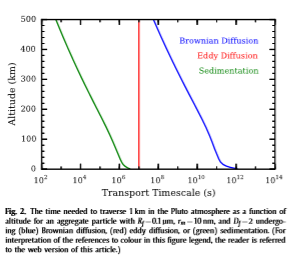
\includegraphics[scale = 1.0]{plt_timescale}
\caption{Transport timescale as modeled using three model dynamics.}
\label{timescale}
\end{figure}
%\begin{thebibliography}{99}

%\bibitem[\protect\citeauthoryear{Allen et al.}{2011}]{Allen+11} Allen, J.~T., Hewett, P.~C., Maddox, N., Richards, G.~T., \& Belokurov, V.\ 2011, MNRAS, 410, 860
%A strong redshift dependence of the broad absorption line quasar fraction
%\bibliography{radio_obser}

%\end{thebibliography}
%\bibliographystyle{unsrt}
%\bibliography{164_final}
%\label{lastpage}

\end{document}